\documentclass{article}
\author{Eric Caleb}
\usepackage{amsmath, amssymb, amsfonts, tikz}
\usepackage{float, geometry}

\date{\today}

\def\standardform#1#2#3{#1x^2 + #2x + #3 = 0}
\def\vertexform#1#2{(#1 - h)^2 + #2 = 0}
\def\interceptform#1#2#3{y = #1(x - #2)(x - #3)}


\begin{document}

\title{Moose Calculations}
\maketitle
\tableofcontents

\pagebreak
\section{Introduction}
In this lab, we will make complex moose calculations using LaTeX.

\section{Equations}

Forms of equations are used to represent relationships between variables. There are several forms of equations, including linear, quadratic, and polynomial equations.
These equatios can also be in different forms, such as standard form, vertex form, or intercept form.
\vspace{1cm}

Standard form: $$\standardform{a}{b}{c}$$
Vertex form: $$\vertexform{h}{k}$$
Intercept form: $$\interceptform{a}{p}{q}$$

Vertex form can be used to find the vertex of a quadratic function. The vertex is the point where the graph of the function crosses the x-axis.
This form is useful with parabolas. An equation in vertex form is of the form $$\vertexform{h}{k}$$, where $(h, k)$ is the vertex of the parabola.

An example parabola in vertex form is $$\vertexform{2}{3}$$, which has vertex $(2, -3)$.

Graphing a parabola in vertex form: $$\vertexform{x}{h}$$

You can graph a parabola in vertex form by finding the vertex and then plotting points on either side of it.
An example graphing a parabola in vertex form is shown below:

\begin{center}
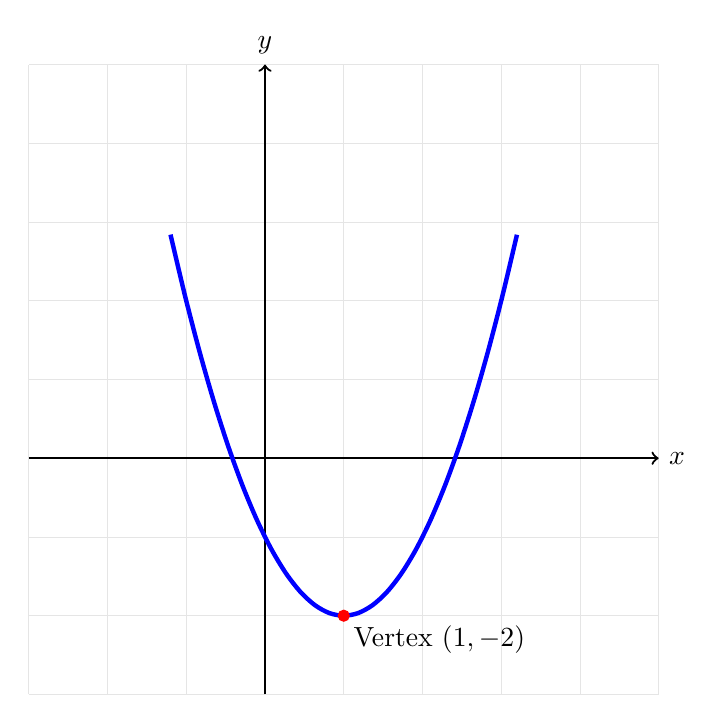
\begin{tikzpicture}
    \draw[step=1cm, gray!20, very thin] (-3,-3) grid (5,5);
    \draw[->, thick] (-3,0) -- (5,0) node[right] {$x$};
    \draw[->, thick] (0,-3) -- (0,5) node[above] {$y$};

    % 2. Plot the Algebraic Function: y = (x - h)^2 + k
    % Change the domain to change how wide the curve stretches.
    % Change '(\x-1)^2 - 2' to match your specific h and k values.
    \draw[
        blue,
        ultra thick,
        smooth,
        variable=\x,
        domain=-1.2:3.2
    ] plot ({\x}, {(\x-1)^2 - 2});

    % 3. Mark the Vertex (h, k)
    \filldraw[red] (1,-2) circle (2pt) node[below right, black] {Vertex $(1,-2)$};

\end{tikzpicture}

\end{center}

\vspace{1cm}

Graphing a parabola in standard form: $$ax^2 + bx + c = 0$$

\begin{center}
    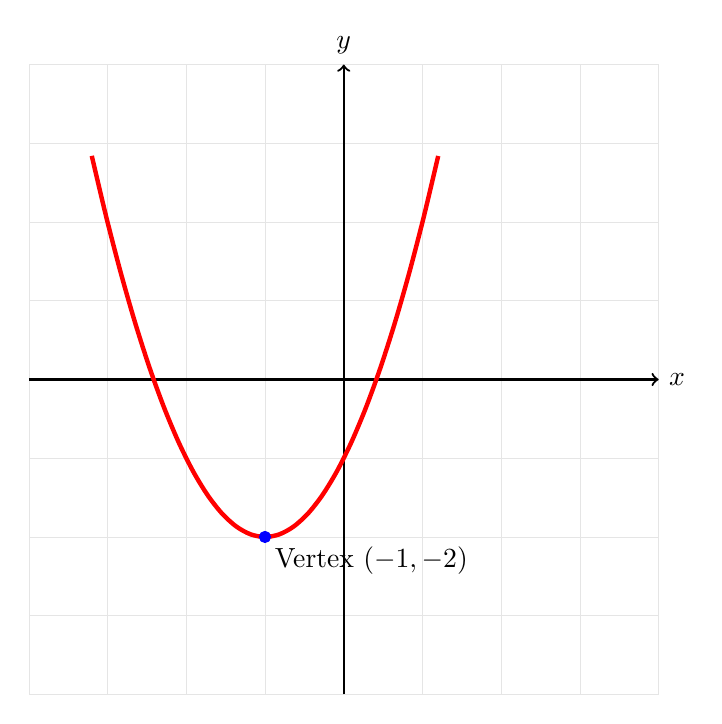
\begin{tikzpicture}
        % 1. Create a background grid and coordinate axes
       \draw[step=1cm, gray!20, very thin] (-4,-4) grid (4,4);
       \draw[->, thick] (-4,0) -- (4,0) node[right] {$x$};
       \draw[->, thick] (0,-4) -- (0,4) node[above] {$y$};

       % 2. Plot the Algebraic Function in Standard Form:  $$ax^2 + bx + c = 0$$
       \draw[
           red,
           ultra thick,
           smooth,
           variable=\x,
           domain=-3.2:1.2
       ] plot ({\x}, {1*(\x)^2 + 2*\x - 1});

       % 3. Mark the calculated vertex (-b/2a, y) -> (-1,-2)
       \filldraw[blue] (-1,-2) circle (2pt) node[below right, black] {Vertex $(-1,-2)$};

    \end{tikzpicture}
\end{center}

Graphing a parabola in intercept form: $$y = a(x-p)(x-q)$$

An example of a parabola in intercept form is $$y = (x-1)(x-5)$$

\begin{center}
    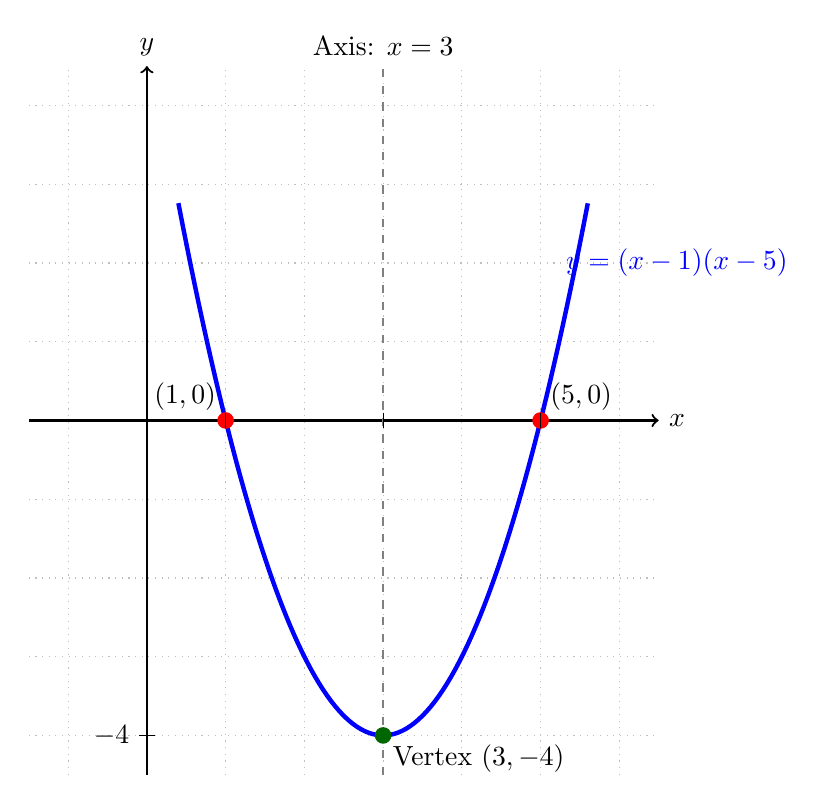
\begin{tikzpicture}
    % Grid lines for background
        \draw[lightgray, dotted, step=1cm] (-1.5,-4.5) grid (6.5,4.5);

        % Axes
        \draw[->, thick] (-1.5,0) -- (6.5,0) node[right] {$x$};
        \draw[->, thick] (0,-4.5) -- (0,4.5) node[above] {$y$};

        % Axis of Symmetry
        \draw[gray, dashed, thick] (3,-4.5) -- (3,4.5) node[above, black] {Axis: $x=3$};

        % Parabola y = (x-1)(x-5) -> y = x^2 - 6x + 5
        \draw[blue, ultra thick, samples=100, domain=0.4:5.6] plot (\x, {\x*\x - 6*\x + 5});
        \node[blue, right] at (5.2,2) {$y = (x-1)(x-5)$};

        % Key Points (Intercepts and Vertex)
        \fill[red] (1,0) circle (3pt) node[above left, black] {$(1,0)$};
        \fill[red] (5,0) circle (3pt) node[above right, black] {$(5,0)$};
        \fill[black!60!green] (3,-4) circle (3pt) node[below right, black] {Vertex $(3,-4)$};

        % Axis tick labels for clarity
        \foreach \x in {1,3,5}
            \draw (\x,0.1) -- (\x,-0.1);
        \foreach \y in {-4}
            \draw (0.1,\y) -- (-0.1,\y) node[left] {$\y$};

    \end{tikzpicture}
\end{center}


Domain of a function is the set of all values of the independent variable for which the function is defined. It usually represents the set of all possible input values.

Range is the set of all values of the dependent variable for which the function is defined. It usually represents the set of all possible output values.

\vspace{1cm}

Equations can be solved using various methods, including factoring, completing the square, and using the quadratic formula.

To solve a quadratic equation of the form $$ax^2 + bx + c = 0$$, use the quadratic formula: $$x = \frac{-b \pm \sqrt{b^2 - 4ac}}{2a}$$.

Solve the equation $$x^2 - 5x + 6 = 0$$ using the quadratic formula.

The solutions are $$x = \frac{5 \pm \sqrt{25 - 24}}{2} = \frac{5 \pm \sqrt{1}}{2}$$.


Solving using factoring: $$x^2 - 5x + 6 = 0 \implies (x-1)(x-6) = 0 \implies x = 1 \text{ or } x = 6$$.

\section{Rectangle}
A rectangle has side lengths $a+4$ and $b+4$. Its area is given by: $$A = (a+4)(b+4)$$.

Perimeter of a rectangle: $$P = 2(a+b)$$.

\section{Centigrade to Fahrenheit}

To convert from centigrade to Fahrenheit, use the formula: $$F = (C \times 9/5) + 32$$.

To convert from Fahrenheit to centigrade, use the formula: $$C = \frac{F - 32}{5/9}$$.

\section{Scientific Notation}

Scientific notation is a way to write very large or very small numbers in a compact form. For example, $1.23 \times 10^5$ is equivalent to $123000$.

To write a number in scientific notation, divide it by the largest power of 10 that divides evenly into it, and write the result with the power of 10 in superscript. For example, $123000$ is written as $1.23 \times 10^5$.

Multiplying numbers in scientific notation involves multiplying the coefficients and adding the exponents. For example, $$2.5 \times 10^3 \times 3.7 \times 10^4$$ is written as $$9.25 \times 10^7$$.

\section{Cirlcle}
The circumference of a circle is given by: $$C = 2 \pi r$$.

The area of a circle is given by: $$A = \pi r^2$$.

\section{Trigonometry}

The sine of an angle is given by: $$\sin \theta = \frac{opposite}{hypotenuse}$$.

The cosine of an angle is given by: $$\cos \theta = \frac{adjacent}{hypotenuse}$$.

The tangent of an angle is given by: $$\tan \theta = \frac{opposite}{adjacent}$$.

\section{Logarithms}

The logarithm of a number is the exponent to which another number must be raised to produce that number. For example, $$\log_2 8 = 3$$ because $2^3 = 8$.

The logarithm of a number with base 10 is called a decimal logarithm, and is denoted by $\log$. For example, $$\log_{10} 100 = 2$$ because $$10^2 = 100$$.

\section{Roots}

The square root of a number is the number that, when multiplied by itself, equals the original number. For example, $$\sqrt{4} = 2$$ because $2^2 = 4$.

The cube root of a number is the number that, when multiplied by itself twice, equals the original number. For example, $$\sqrt[3]{27} = 3$$ because $3^3 = 27$.

The fourth root of a number is the number that, when multiplied by itself three times, equals the original number. For example, $$\sqrt[4]{16} = 2$$ because $2^4 = 16$.

Algebra roots are used to solve equations of the form $$x^n = a$$, where $n$ is the root and $a$ is the number.

For example, $$x^3 = 27$$ has a cube root of $$\sqrt[3]{27} = 3$$.

Algebraic fractions can be used to solve equations of the form $$\frac{x^n}{a} = b$$, where $n$ is the root, $a$ is the numerator, and $b$ is the denominator. For example, $$\frac{x^2}{3} = 4$$ has a square root of $$\sqrt[2]{4} = 2$$.

\section{Distributive Property}

Distributive property is used to simplify expressions and solve equations.
The distributive property states that $$a(b + c) = ab + ac$$ for all numbers $a$, $b$, and $c$ \in $\mathbb{R}$.  For example, $$2(3 + 4) = 2 \times 3 + 2 \times 4 = 6 + 8 = 14$$.


\section{Sets}

Sets are collections of objects or numbers. For example, $$\{1, 2, 3\}$$ is a set of three numbers.

Sets can be represented using set notation, which uses curly braces to enclose the elements of the set. For example, $$\{a, b, c\}$$ is a set of three letters.

Sets can be used to represent the solutions to equations and inequalities. For example, $$\{x \in \mathbb{R} : x^2 < 5\}$$ is the set of all real numbers $x$ such that $x^2 < 5$.

\section{Fractions}

Fractions are used to represent parts of a whole. A fraction $$\frac{a}{b}$$ has a numerator $a$ and a denominator $b$. For example, $$\frac{1}{2}$$ is a fraction with a numerator of 1 and a denominator of 2.

Fractions can be added, subtracted, multiplied, and divided to solve equations and inequalities.

Fractions can be simplified by finding the greatest common divisor (GCD) of the numerator and denominator and dividing both by it. For example, $$\frac{6}{12} = \frac{1}{2}$$.

Fractions can be used in algebra to solve equations and inequalities.

For example, $$\frac{1}{x} + \frac{1}{x} = \frac{2}{x}$$ can be simplified to $$\frac{2}{x} = 1$$.

Another example is $$2\left(\frac{1}{x^2-1}\right) = 1$$, which we can solve for x by multiplying both sides by $$\frac{1}{2}$$ to get $$\frac{1}{x^2-1} = 1$$, and then solving for x.
The solution is $$x = \pm 3$$.

Complex fractions can be simplified using the same methods as regular fractions. For example, $$\frac{1}{a+bi} = \frac{a}{a^2+b^2} + \frac{b}{a^2+b^2}i$$.


\section{Vectors}

Vectors are used to represent quantities that have both magnitude and direction. For example, a velocity vector has a magnitude (speed) and a direction (e.g. north, south, east, west).
Vectors can be added, subtracted, and multiplied to solve equations and inequalities.

An example of a vector equation is $$\vec{v} = \vec{a} + \vec{b}$$, where $\vec{v}$ is the resultant vector, $\vec{a}$ is the first vector, and $\vec{b}$ is the second vector.

\section{Tabular data}

Tabular data can be displayed using the `tabular` environment. For example a table of values for $f(x)$ can be displayed as follows:

\begin{table}[H]
\centering
\def \arraystretch{2}
\begin{tabular}{||c|c|}
    \hline
    x & f(x) \\
    \hline
    1 &  2 \\
    \hline
    2 &  4 \\
    \hline
    3 &  6 \\
    \hline
    4 &  8 \\
    \hline
    $\frac{1}{2}$ &  $\frac{1}{4}$ \\
    \hline


\end{tabular}
\caption{Table of values for $f(x)$}
\label{tab:f(x)}

\end{table}

\end{document}
